\documentclass{report}
\usepackage[a4paper,margin=0.4in,bottom=0.7in]{geometry}
\usepackage{graphicx,wrapfig,amsmath,amssymb,algorithm,algpseudocode,caption,subcaption,xcolor} 

\title{Digital Image Processing}
\author{Abhijit Amrendra Kumar}
\date{August 2023}

\setlength\parindent{0pt}

\begin{document}
\maketitle

\chapter{Image Warping and Alignment}
\section{Basics}

A digital image, which is a version of the visual stimulus sampled at discrete locations with discretized values, can be regarded as a function $I = f(x,y)$, where $(x,y)$ are the spatial integer coordinates in typically a rectangular domain $\Omega = [0,W-1]\times[0,H-1]$. Each ordered pair $(x,y)$ denote a pixel, which is generally a square. Pixel dimensions relate to the spatial resolution of the light-collecting sensor of a camera. \\

The actual visual signal is analog, but digital cameras capture a discrete version of it, and also quantize the intensity values. In a typical grayscale image, the intensity values lie from $0\rightarrow 255$

\begin{center}
  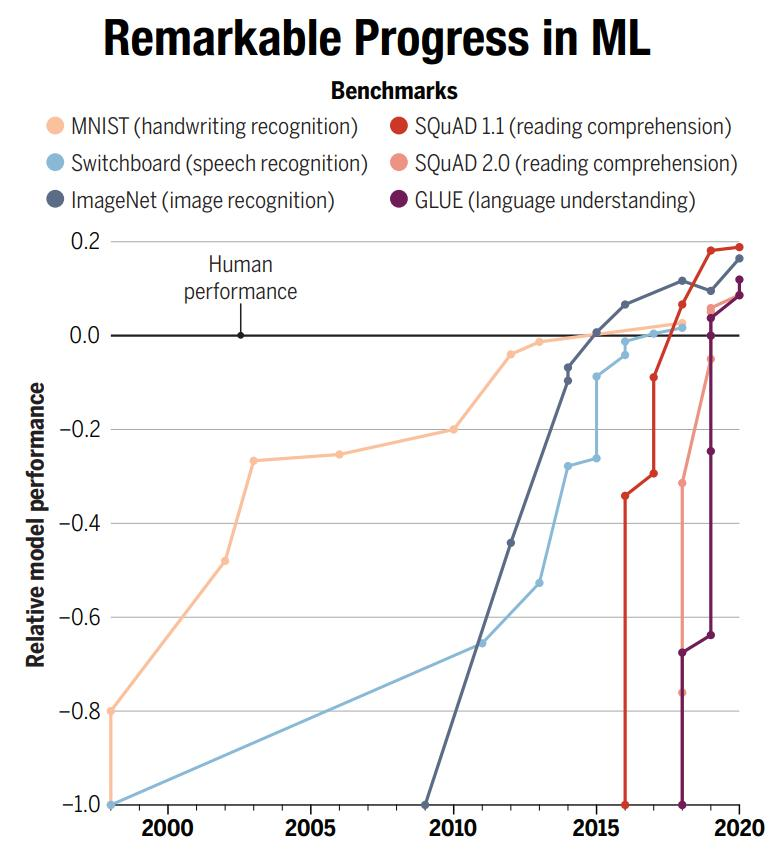
\includegraphics[scale=0.5]{"images/01.png"}
\end{center}

\section{Alignment}

Consider images $I_1,I_2$ of a scene acquired through different viewpoints. $I_1$ and $I_2$ are said to be aligned iff for every $(x,y)$ in the domain $\Omega$, the pixels at $(x,y)$ in $I_1$ and $I_2$ are in physical correspondence. \\

If not, the images are said to be misalgined with respect to each other, or we say there is relative motion between the images. Image alignment is the process of correcting for the relative motion between $I_1$ and $I_2$.

\newpage
\section{Motion Models}

Let us denote the coordinates in $I_1$ as $(x_1,y_1)$, and those in $I_2$ as $(x_2,y_2)$. \\

Let's first consider \textbf{translation}.

\begin{align}
  \forall (x_1,y_1) \in \Omega, & \exists t_x,t_y, x_2 = x_1 + t_x, y_2 = y_1 + t_y \\
  \implies \begin{bmatrix}
             x_2 \\
             y_2 \\
             1
           \end{bmatrix}
                                & = \begin{bmatrix}
                                      1 & 0 & t_x \\
                                      0 & 1 & t_y \\
                                      0 & 0 & 1
                                    \end{bmatrix} \begin{bmatrix}
                                                    x_1 \\
                                                    y_1 \\
                                                    1
                                                  \end{bmatrix}
\end{align}

Next, let's consider rotation about a point $(x_c,y_c)$ anti-clockwise through angle $\theta$

\begin{align}
  x_2 & = (x_1-x_c)\cos\theta - (y_1-y_c)\sin\theta + x_c \\
  y_2 & = (x_1-x_c)\sin\theta + (y_1-y_c)\cos\theta + y_c \\
      & \implies \begin{bmatrix}
                   x_2 \\
                   y_2 \\
                   1
                 \end{bmatrix}
  = \begin{bmatrix}
      \cos\theta & -\sin\theta & x_c \\
      \sin\theta & \cos\theta  & y_c \\
      0          & 0           & 1
    \end{bmatrix} \begin{bmatrix}
                    x_1-x_c \\
                    y_1-y_c \\
                    1
                  \end{bmatrix}
\end{align}

Combining the two motions, we obtain
\begin{align}
  x_2 & = (x_1-x_c)\cos\theta - (y_1-y_c)\sin\theta + t_x \\
  y_2 & = (x_1-x_c)\sin\theta + (y_1-y_c)\cos\theta + t_y \\
      & \implies \begin{bmatrix}
                   x_2 \\
                   y_2 \\
                   1
                 \end{bmatrix}
  = \begin{bmatrix}
      \cos\theta & -\sin\theta & t_x \\
      \sin\theta & \cos\theta  & t_y \\
      0          & 0           & 1
    \end{bmatrix} \begin{bmatrix}
                    x_1-x_c \\
                    y_1-y_c \\
                    1
                  \end{bmatrix}
\end{align}

If the $2\times 2$ matrix $\begin{bmatrix}
    A_{11} & A_{12} \\
    A_{21} & A_{22} \\
  \end{bmatrix}$ is rank-deficient, we term the transformation as an \textbf{affine transformation}, since it will transform 2D figures into a line/point. \\

\textbf{Note}: Composition of multiple types of motion is given by the multiplication of their corresponding matrices. However, most motion compositions are not commutative.

\begin{center}
  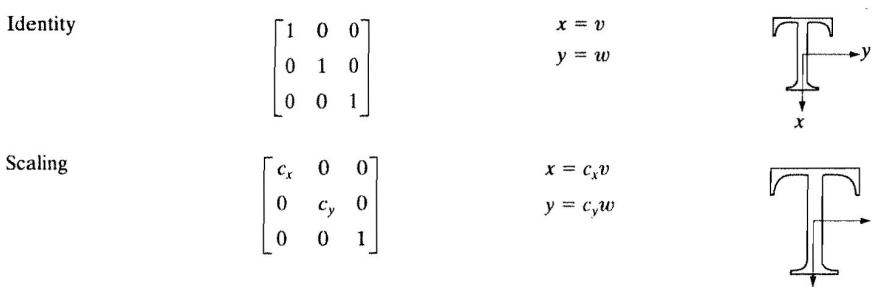
\includegraphics[scale=0.8]{"images/02.png"}
  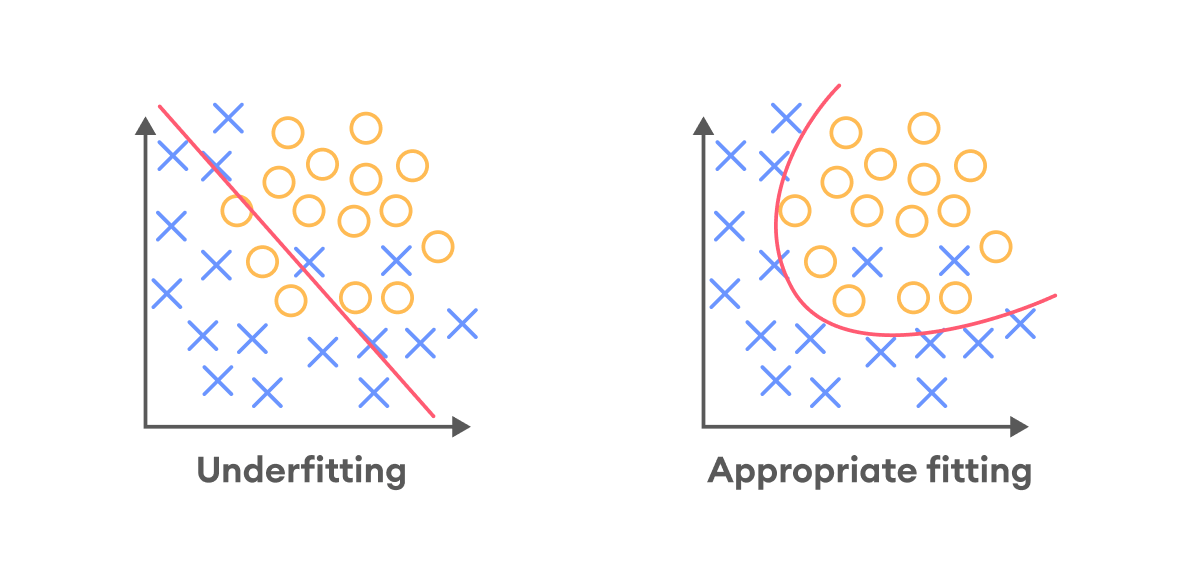
\includegraphics[scale=0.9]{"images/03.png"}
\end{center}

\section{Image Alignment: Control Points}

This method involves marking pairs of physically corresponding points on two images, either manually by an expert or automatically using geometric properties. Then using these points, the transformation matrix can be computed, and the whole image can be transformed to align with the original image.

\begin{center}
  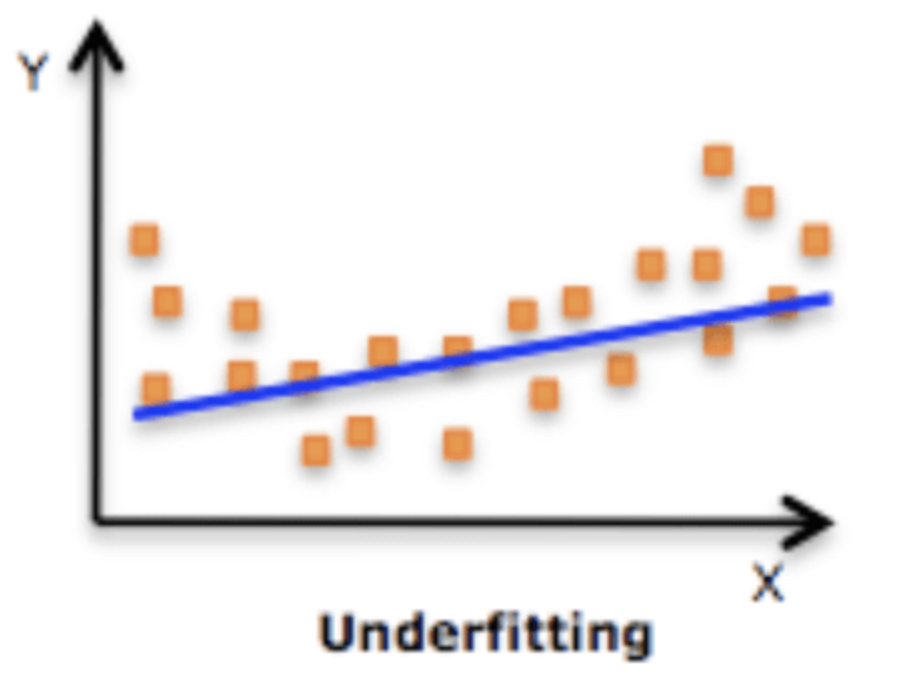
\includegraphics[scale=1]{"images/04.png"}
\end{center}

The matrix equation obtained by this method is as follows:
$$
  \begin{bmatrix}
    x_{21} & x_{22} & \ldots & x_{2N} \\
    y_{21} & y_{22} & \ldots & y_{2N} \\
    1      & 1      & \ldots & 1
  \end{bmatrix} =
  \begin{bmatrix}
    A_{11} & A_{12} & t_x \\
    A_{21} & A_{22} & t_y \\
    0      & 0      & 1   \\
  \end{bmatrix}
  \begin{bmatrix}
    x_{11} & x_{12} & \ldots & x_{1N} \\
    y_{11} & y_{12} & \ldots & y_{1N} \\
    1      & 1      & \ldots & 1
  \end{bmatrix}
$$

In shorthand, we can denote it as
$$
  P_2 = TP_1
$$

Since $P_1$ can be possibly rank deficient, we can instead minimize $||P_2-TP_1||^2_2$, the solution to which is
$$
  T = P_2 \operatorname{pinv}(P_1)
$$

However, this method is always not feasible, because
\begin{itemize}
  \item it requires manual intervention
  \item it is error prone
  \item there are automatic methods like the SIFT technique to finding matching control points.
\end{itemize}

\section{Image Alignment: Mean Squared Error}

The mean squared error between 2 images is given by
$$
  \text{MSSD} = \frac{1}{N} \underset{x,y\in\Omega}{\sum} (I_1(x,y)-I_2(x,y))^2, \ N = \#\text{pixels in field of view}
$$

We can modify the equation in the following manner to find the transform matrix $T$
$$
  T^* = \underset{T}{\text{argmin}} \operatorname{MSSD}(I_1(v), I_2(Tv)), \quad
  v = \begin{bmatrix}
    x \\
    y \\
    1
  \end{bmatrix},
  T = \begin{bmatrix}
    A_{11} & A_{12} & t_x \\
    A_{21} & A_{22} & t_y \\
    0      & 0      & 1   \\
  \end{bmatrix}
$$

Assuming a simple model involving translation and rotation,
$$
  T = \begin{bmatrix}
    \cos\theta & -\sin\theta & t_x \\
    \sin\theta & \cos\theta  & t_y \\
    0          & 0           & 1   \\
  \end{bmatrix}
$$

The simplest (although the worst possible way) to solve this would be to iterate over ranges for $\theta,t_x,t_y$.

\subsection{Image Warping}

Applying the transformation $T$ over an image maps each coordinate vector $v = [x,y]$ to the new coordinate $Tv$ in the new image, where $x,y \in \mathbb{Z}$. However, it is very likely that $Tv = [x',y']$ does not consist of integer coordinates.
This transformation, also known as \textbf{forward warping}, can lead to holes in the new image, and can also lead to multiple intensity values if the image is scaled down. \\

Instead, we can use \textbf{reverse warping}, which involves taking $v' = [x',y'], x',y' \in \mathbb{Z}$ in the new image, and applying the inverse transformation $T^{-1}v$ to get the coordinates in the original image. Here, if $T^{-1}v$ does not consist of integer coordinates, we can use methods like bilinear interpolation or nearest neighbour to calculate the intensity value to be used from the original image.

\begin{center}
  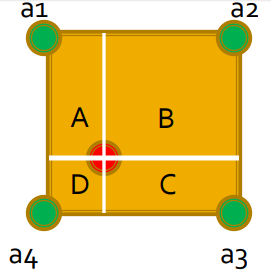
\includegraphics[scale=0.8]{"images/05.png"} \qquad
  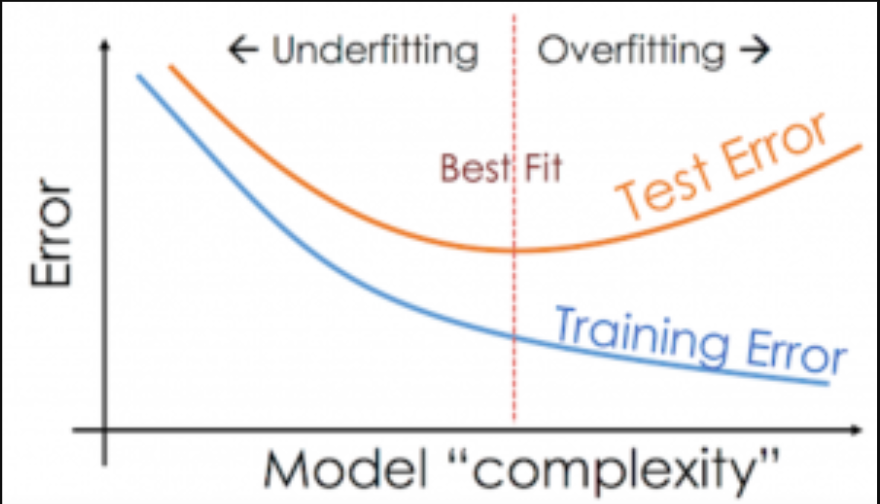
\includegraphics[scale=1.1]{"images/06.png"}
\end{center}

\textbf{Nearest Neighbour}: Pick $a_4$ \\

\textbf{Bilinear interpolation}: Use the following value (weights being the areas of the 4 regions)
$$
  \frac{Ba_4 + Aa_3 + Ca_1 + Da_2}{A+B+C+D} = Ba_4 + Aa_3 + Ca_1 + Da_2 \qquad (A+B+C+D = 1 \text{ for unit pixel})
$$

Essentially, we have to find the following function
$$
  f(x,y) = a_0 + a_1x + a_2y + a_3xy
$$

To determine the coefficients, we can solve the following equation
$$
  \begin{bmatrix}
    1 & x_1 & y_1 & x_1y_1 \\
    1 & x_1 & y_2 & x_1y_2 \\
    1 & x_2 & y_1 & x_2y_1 \\
    1 & x_2 & y_2 & x_2y_2
  \end{bmatrix}
  \begin{bmatrix}
    a_0 \\
    a_1 \\
    a_2 \\
    a_3
  \end{bmatrix} =
  \begin{bmatrix}
    f(x_1,y_1) \\
    f(x_1,y_2) \\
    f(x_2,y_1) \\
    f(x_2,y_2)
  \end{bmatrix}
$$

$$
  \implies
  \begin{bmatrix}
    a_0 \\
    a_1 \\
    a_2 \\
    a_3
  \end{bmatrix} =
  \begin{bmatrix}
    1 & x_1 & y_1 & x_1y_1 \\
    1 & x_1 & y_2 & x_1y_2 \\
    1 & x_2 & y_1 & x_2y_1 \\
    1 & x_2 & y_2 & x_2y_2
  \end{bmatrix}^{-1}
  \begin{bmatrix}
    f(x_1,y_1) \\
    f(x_1,y_2) \\
    f(x_2,y_1) \\
    f(x_2,y_2)
  \end{bmatrix}
$$
\vspace{5mm}

\textbf{{\color{blue} Note}}: Alignment with MSSD relies heavily on the fact that the intensity for physically corresponding points is the same. However, we can have images of the same physical entity from different sensors or lighting conditions. \\

\textbf{\color{red} Caution}: When an image is rotated, because of the rectangular shape of an image, the rotated image will have some black regions, which denote the area which is outside the field of view.
\begin{center}
  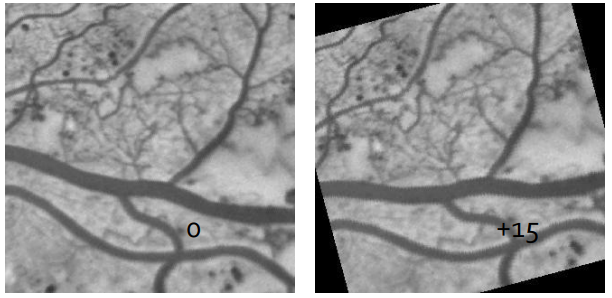
\includegraphics[scale=0.7]{"images/07.png"}
\end{center}

We need to compute the MSSD only over the overlapping region between the two images.

\section{Alignment with Differing Intensities}

% ----------------------------------------------------------------

\chapter{Edge and Corner Detection}

\textbf{Edge pixels} are those at which image intensity changes abruptly.

\textbf{Edge segments} or edges are sets of connected edge pixels

\section{Digital Derivatives}

Along a ramp, first derivative is a non-zero constant, while the second derivative is zero along the ramp (except the start and end).

% ----------------------------------------------------------------

\chapter{Hough Transform}

A hough transform is a method used to detect the presence of different types of shapes in an image. This can be extended to detect important features in an image, like roads and buildings in satellite imagery, biological cells in microscope images, etc.
\begin{center}
  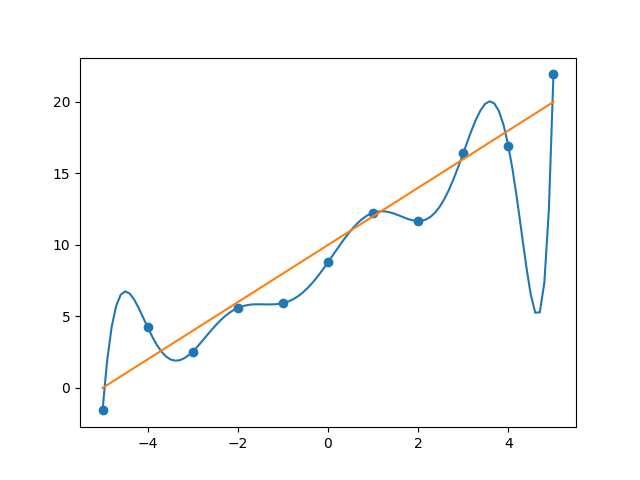
\includegraphics[scale=0.77]{"images/08.png"} \qquad
  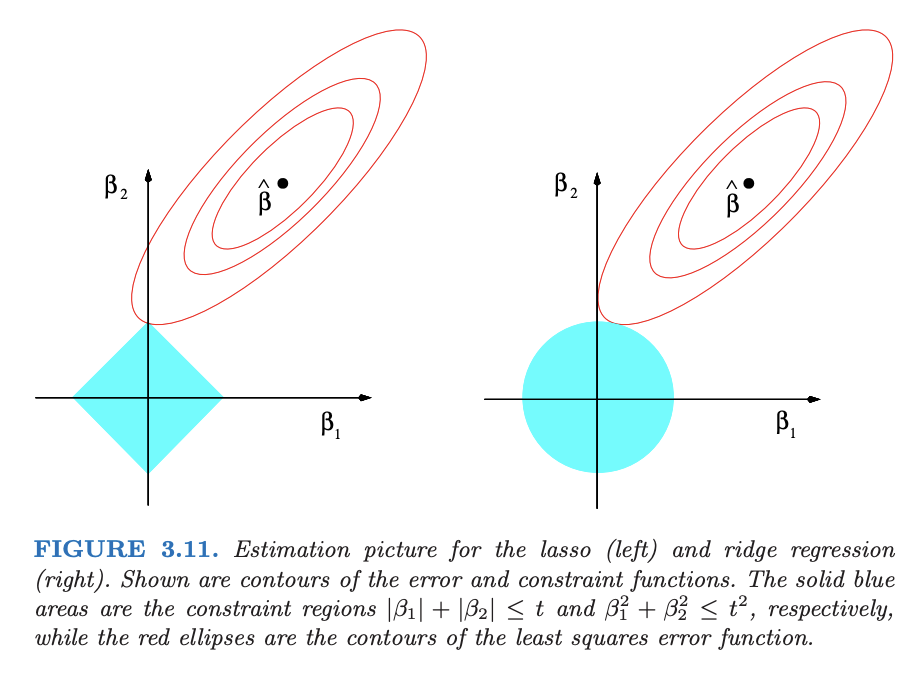
\includegraphics[scale=0.8]{"images/09.png"}
\end{center}

\section{Line Detection}

Consider a point $(x_i,y_i)$ in the image. A line passing through it can be represented by $y_i = ax_i + b$, which is parametrized by $(a,b)$. Thus, each line becomes a point $(a,b)$ in the \textbf{parameter space}. The set of all lines passing through $(x_i,y_i)$ will constitute a single line in the parameter space.

However, this slope intercept form for the parameter space can prove challenging to execute, since slopes can be unbounded. Instead, we can use the normal representation
$$
  x\cos\theta + y\sin\theta = p
$$

Thus, a single point in the $XY$ space corresponds to a \textbf{sinusoid} in this parameter space. The line joining two points in the $XY$ space is represented by a point obtained from the intersection of their corresponding two sinusoids in the parameter space.

\subsection{Algorithm}
\begin{itemize}
  \setlength\itemsep{0mm}
  \item Divide the entire $(p,\theta)$ space into a 2D array of bins.
  \item For every point $(x_k,y_k)$ in the $XY$ space, and for every value of $\theta$ from $-90$ to $90$, compute the corresponding value of $p$ using $p = x_k\cos\theta + y_k\sin\theta$.
  \item Approximate this value to the closest allowed cell value in the $(p,\theta)$ space.
  \item Increment the frequency count of that cell by 1 (voting).
  \item Finally, pick those lines having maximum votes
\end{itemize}
\vspace{4mm}

\begin{center}
  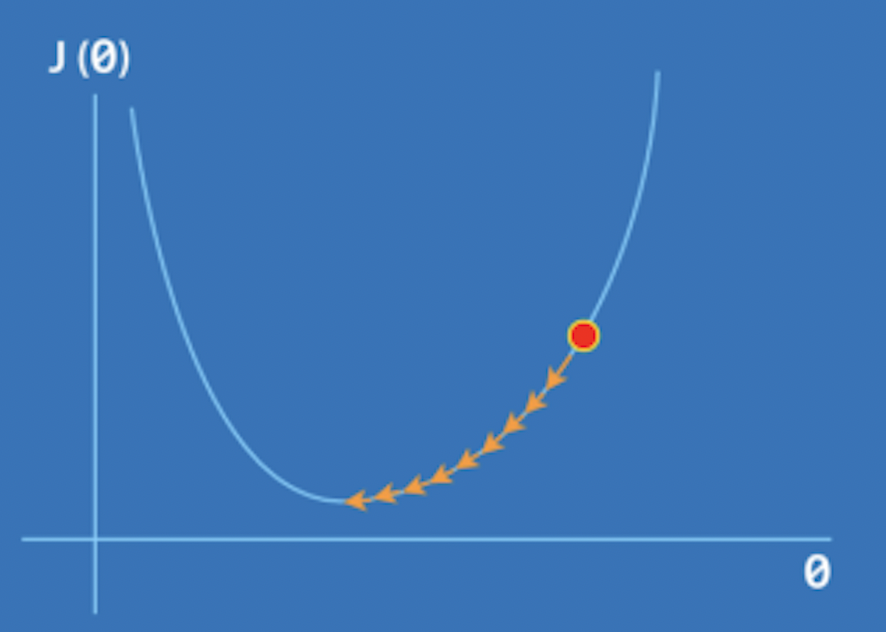
\includegraphics[scale=0.6]{"images/11.png"}
  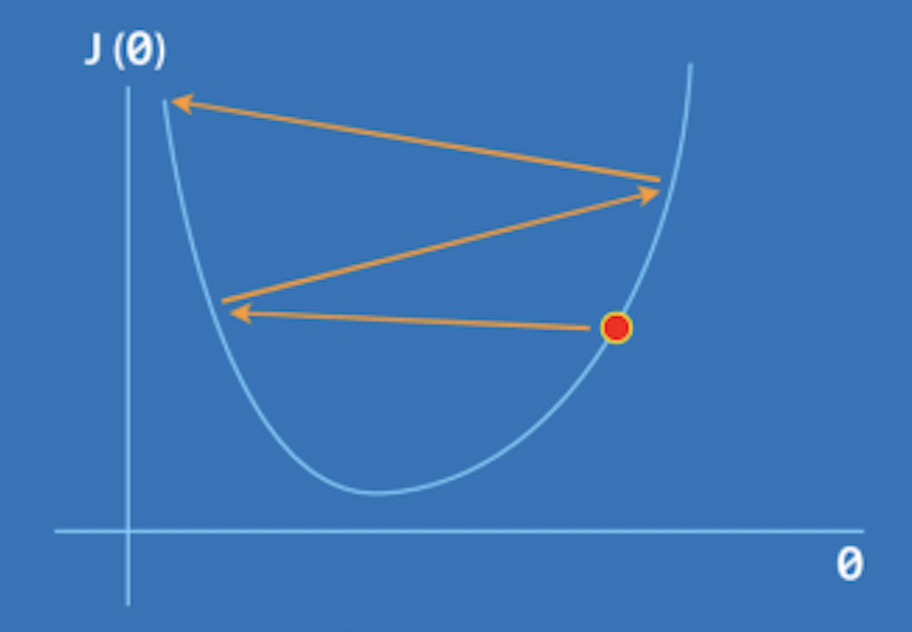
\includegraphics[scale=0.6]{"images/12.png"}
\end{center}

Here's an example from Wikipedia
\begin{center}
  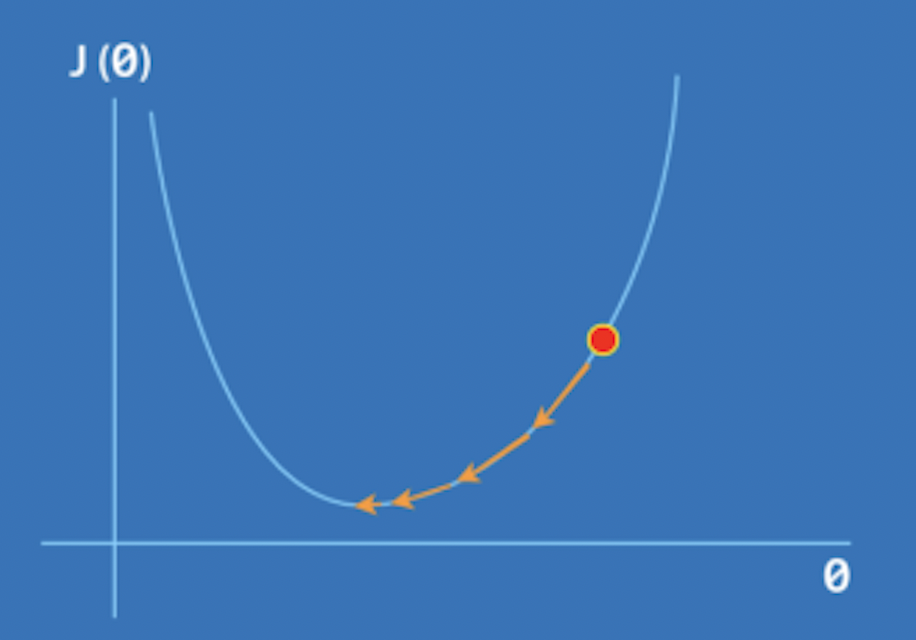
\includegraphics[scale=0.35]{"images/10.png"}
\end{center}

\subsection{Speed-up Heuristic}

Computing the gradient for each point, we know that the edge direction should be approximately perpendicular to the gradient. \\

Therefore, given the edge direction $\theta'$, we can iterate over $\theta$ from $\theta'-K$ to $\theta'+K$, $K$ being around $20$ degrees.

\section{Circle and Ellipse Detection}

A circle is represented by the equation $(x-a)^2 + (y-b)^2 = r^2$, and so is characterized by 3 parameters $(a,b,r)$. Thus, the parameter space is 3D, and we can use the same iterative algorithm. Similarly, the parameter space for an ellipse whose axes are parallel to the $XY$ axes is 4D, while it is 5D for a general ellipse.

\section{Pros}
\begin{itemize}
  \item It can even handle cases for a broken shape (gaps in the shape perimeter) caused by occlusions or noise.
\end{itemize}

\section{Cons}
\begin{itemize}
  \item Exponential computational complexity in the number of parameters
  \item It considers a line to be of infinite extent, hence relatively smaller line segments can get missed out.
  \item Low image resolution can lower the accuracy of this algorithm, as potentially different curves could fall into the same bins. Even very high resolution images can be problematic, as votes of different points lying close to the same curve will get bifurcated. Also, noise worsens the accuracy in the latter case.
\end{itemize}

\end{document}
